\documentclass{article}
\usepackage{tikz}


\begin{document}
    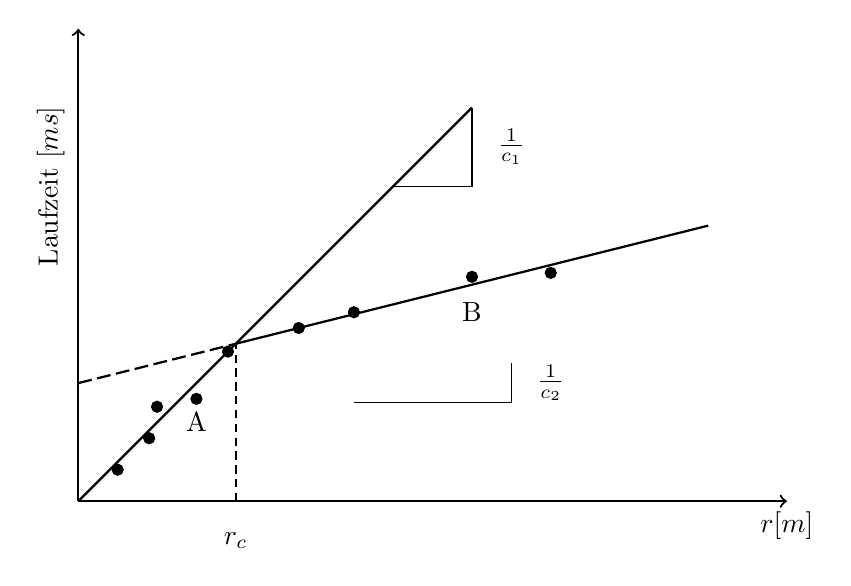
\begin{tikzpicture}
        
        %Diagramm
        \draw[->, thick] (0,0) -- (0, 6) node[rotate = 90] at (-0.35, 4) {Laufzeit $[ms]$};
        \draw[->, thick] (0,0) -- (9,0) node[below] {$r[m]$};

        \draw[black, thick, domain = 0:5] plot (\x,  \x) ;
        \draw[black, thick, dash pattern = {on 5pt off 2pt}, domain = 0:2] plot (\x, {0.25*\x + 1.5});
        \draw[black, thick, domain = 2:8] plot (\x, {0.25*\x + 1.5});
        \draw[black, thick, dash pattern = {on 3pt off 2pt}] (2,0) -- (2,2);

        %Steigung
        \draw[black, thin] (4, 4) -- (5, 4) -- (5, 5);
        \draw[black, thin] (3.5, 1.25) -- (5.5, 1.25) -- (5.5, 1.75);

        %Nodes
        \node at (5.5, 4.5) {$\frac{1}{c_1}$};
        \node at (6, 1.5) {$\frac{1}{c_2}$};
        \node at (2, -0.5) {$r_c$};
        \node at (1.5, 1) {A};
        \node at (5, 2.4) {B};

        %Punkte
        \filldraw[black] (0.5, 0.4) circle (2pt);
        \filldraw[black] (0.9, 0.8) circle (2pt);
        \filldraw[black] (1, 1.2) circle (2pt);
        \filldraw[black] (1.5, 1.3) circle (2pt);
        \filldraw[black] (1.9, 1.9) circle (2pt);
        \filldraw[black] (2.8, 2.2) circle (2pt);
        \filldraw[black] (3.5, 2.4) circle (2pt);
        \filldraw[black] (5, 2.85) circle (2pt);
        \filldraw[black] (6, 2.9) circle (2pt);

    \end{tikzpicture}
\end{document}
